\chapter{Ongelmat JavaScriptin staattisessa tyypittämisessä}

\section{EcmaScript-yhteensopivuus}

TypeScript pyrkii noudattamaan mahdollisimman 
tarkasti EcmaScript-spesifikaatiota kaikkien sellaisten
ominaisuuksien suhteen jotka
eivät nimenomaan liity staattiseen tyypittämiseen. 

Todo

\section{Tyyppien automaattinen ja vaiheittainen tyypittäminen}

Todo

\section{Luotettavuus, täydellisyys ja käytännöllisyys}

\begin{figure}
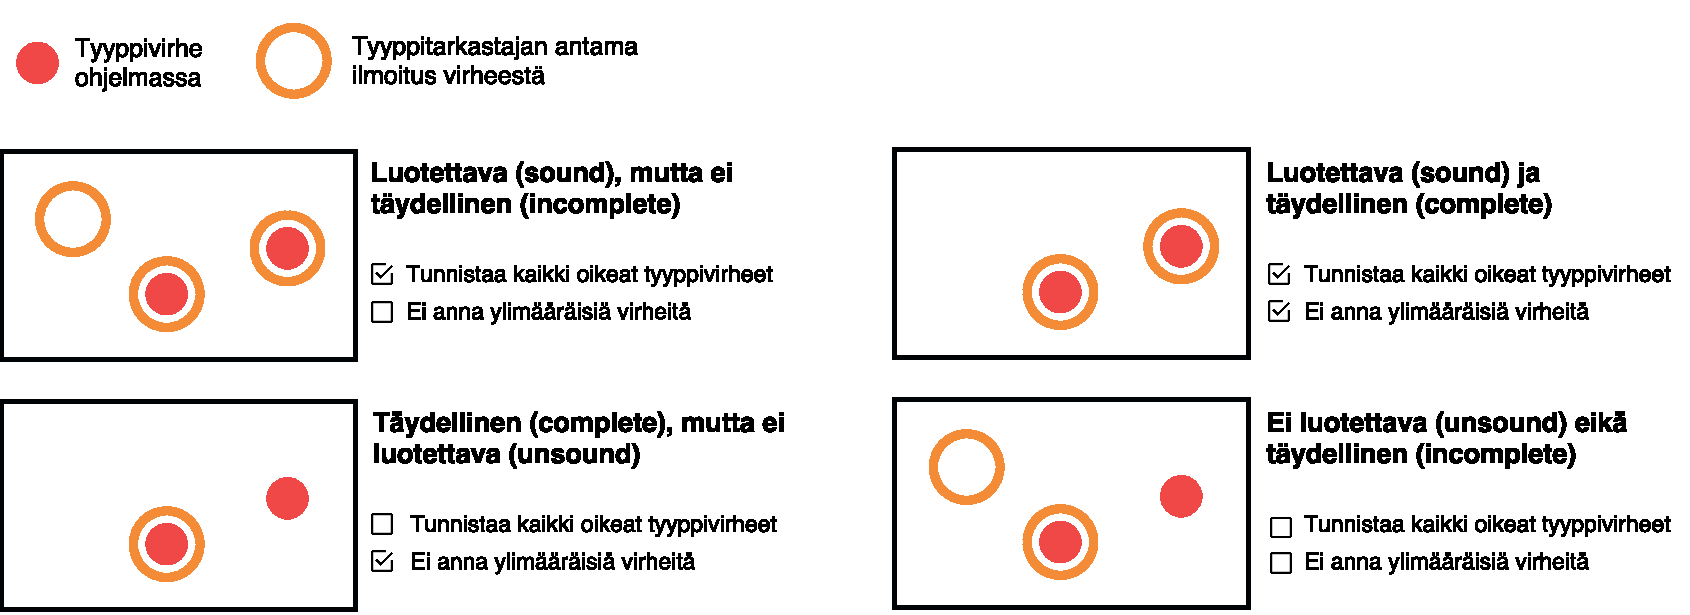
\includegraphics[width=\textwidth]{images/soundness_completeness2.pdf}
\caption{Tyyppijärjestelmän luotettavuus ja täydellisyys}
\end{figure}

Tyyppijärjestelmän luotettavuus (soundness) kuvaa sitä, kuinka suuren osan
mahdollisista ohjelmointivirheistä se estää. Täysin luotettava (sound)
tyyppijärjestelmä estää kaikki sellaiset virheet jotka sen on tarkoitus
estää \cite{CSE_ProgrammingLanguages}. Täydellisyys (completeness)
puolestaan kertoo salliiko tyyppijärjestelmä kielen sellaiset ominaisuudet
jotka eivät olisi ajonaikana tyyppivirheitä \cite{TypesAndProgrammingLanguages, CSE_ProgrammingLanguages}.

Jotta JavaScriptiä analysoiva tyyppijärjestelmä olisi luotettava, sen on
annettava virhe esimerkiksi seuraavasta ohjelmasta:

\begin{minipage}{\linewidth}
\begin{lstlisting}[caption={Virheellinen JavaScript-ohjelma: Lisätyllä tuotteella ei ole nimeä.}]
function osta(ostos) {
  lisaaTuote({
    nimi: ostos.nimi,
    hinta: ostos.hinta
  });
}

osta({ nimi: 'juusto', hinta: 5 });
osta({ hinta: 5 });
\end{lstlisting}
\label{fig:soundness_test}
\end{minipage}

Toisaalta jotta JavaScriptiä analysoiva tyyppijärjestelmä olisi täydellinen,
sen on sallittava tämä korjattu versio ylläolevasta ohjelmasta:

\begin{minipage}{\linewidth}
\begin{lstlisting}[caption={Toimiva JavaScript-ohjelma: Virheelliseltä kutsulta on suojauduttu tarkistuksella.}]
function osta(ostos) {
  if (typeof ostos.nimi === 'string') {
    lisaaTuote({
      nimi: ostos.nimi,
      hinta: ostos.hinta
    });
  }
}

osta({ nimi: 'juusto', hinta: 5 });
osta({ hinta: 5 });
\end{lstlisting}
\label{fig:completeness_test}
\end{minipage}

Esimerkit \ref{fig:soundness_test} ja \ref{fig:completeness_test} toimivat
odotetulla tavalla Flow:ssa. TypeScript vaatii eksplisiittisen tyyppiannotaation
osta-funktiolle, mutta toimii muuten samalla tavalla. Flow, TypeScript ja
Closure eivät kuitenkaan ole täydellisiä tai kokonaan luotettavia.
Monimutkaisemmissa tilanteissa virheitä saattaa jäädä nappaamatta tai toimiva
ohjelma voidaan merkata virheelliseksi. JavaScriptiä käännöskohteena käyttävät
mutta muuten sen syntaksista ja semantiikasta eroavat uudet kielet,
kuten Dart ja Elm, on voitu kehittää toivotunlaiseksi ilman painetta olla
yhteensopiva vanhan koodin kanssa.

TypeScript ja Flow on sen sijaan kehitetty lisäämään staattinen tyypitys
olemassa olevaan kieleen, JavaScriptiin, siten että nykyisellään käytössä
olevat kirjastot ja koodikäytännöt pystytään tyyppitarkastamaan ilman että
niiden arkkitehtuuria tarvitsee merkittävästi muuttaa tyyppiturvallisuuden
saavuttamiskesi.

TypeScript on strukturaalisesti tyypitetty, minkä vuoksi seuraava koodi kääntyy
ilman tyyppivirheitä.

\begin{minipage}{\linewidth}
\begin{lstlisting}[caption={Loogisen virheen sisältävä, mutta ilman virheitä kääntyvä TypeScript-ohjelma.}]
class Ihminen {
    constructor(public nimi: string){}
}

class Elain {
    constructor(public nimi: string){}
}

function varaaAikaElainlaakariin(omistaja: Ihminen, lemmikki: Elain) { }

varaaAikaElainlaakariin(new Elain("Musti"), new Ihminen("Jaakko"));
\end{lstlisting}
\label{fig:structural_typing_error}
\end{minipage}

TypeScript kääntäjä sallii esimerkin \ref{fig:structural_typing_error} koodin
vaikka funktion arugmentit "omistaja" ja "lemmikki" ovat väärin päin, sillä
molempien luokkien rakenne on sama, molemmissa on pelkkä tekstimuotoinen
ominaisuus "name". Flow:ssa sama virhe ei menisi läpi, sillä siinä luokkainstanssit
on tyypitetty nominaalisesti, mikä auttaa tässä esimerkissä mutta aiehuttaa ongelmia
muissa tilanteissa. Projekti saattaa esimerkiksi sisältää kaksi versiota samasta
kirjastosta jonkin toisen kirjaston kautta, mikä voi aiheuttaa yhteensopimusongelmia
kun käytännössä saman luokan tyyppejä ei lueta keskenään yhteensopiviksi. 